\documentclass{ctexart}
\usepackage{siunitx}
\usepackage[a4paper,top=1.5cm,bottom=1.5cm,left=2cm,right=2cm]{geometry}
\usepackage{graphicx}
\usepackage{theorem}
{
	\theoremstyle{change}
	\theoremheaderfont{\bfseries}
	\theorembodyfont{\normalfont}
	\newtheorem{ti}{}[section]
}
\renewcommand{\theti}{\arabic{ti}.}
\usepackage{paralist}
\renewcommand{\theenumi}{\arabic{enumi}}
\renewcommand{\labelenumi}{(\theenumi)}
\setCJKmainfont{SourceHanSerifCN-Regular}

\title{《数字电子技术基础》2018-2019 第二学期考试卷\thanks{试卷编号:1819020603A,电气专业考试}}
\author{秦舒雅}
\begin{document}
	\pagestyle{plain}
	\maketitle
	此文档为“临时”文档,应朋友之邀匆忙整理出此文档,图均为手画,内容也不是全的,待我有空去学画电路图时,再重新编排。
	\begin{ti}[$6$ 分]
		求原码、补码
		\[
			-15,-101111
		\]
	\end{ti}

	\begin{ti}[$12$ 分]
		画出卡诺图
		\[
			Y = \sum m(0,1,2,3,4,6,8,9,10,11,14)
		\]
	\end{ti}

	\begin{ti}[$9$ 分]
		图~\ref{fig:1}、\ref{fig:2} 由 TTL 构成,图~\ref{fig:3} 由 CMOS 门电路构成,写出 $F_{1},F_{2},F_{3}$ 的表达式
		\begin{figure}[htbp]
			\centering
			\parbox[t]{0.5\textwidth}{%
				\centering
				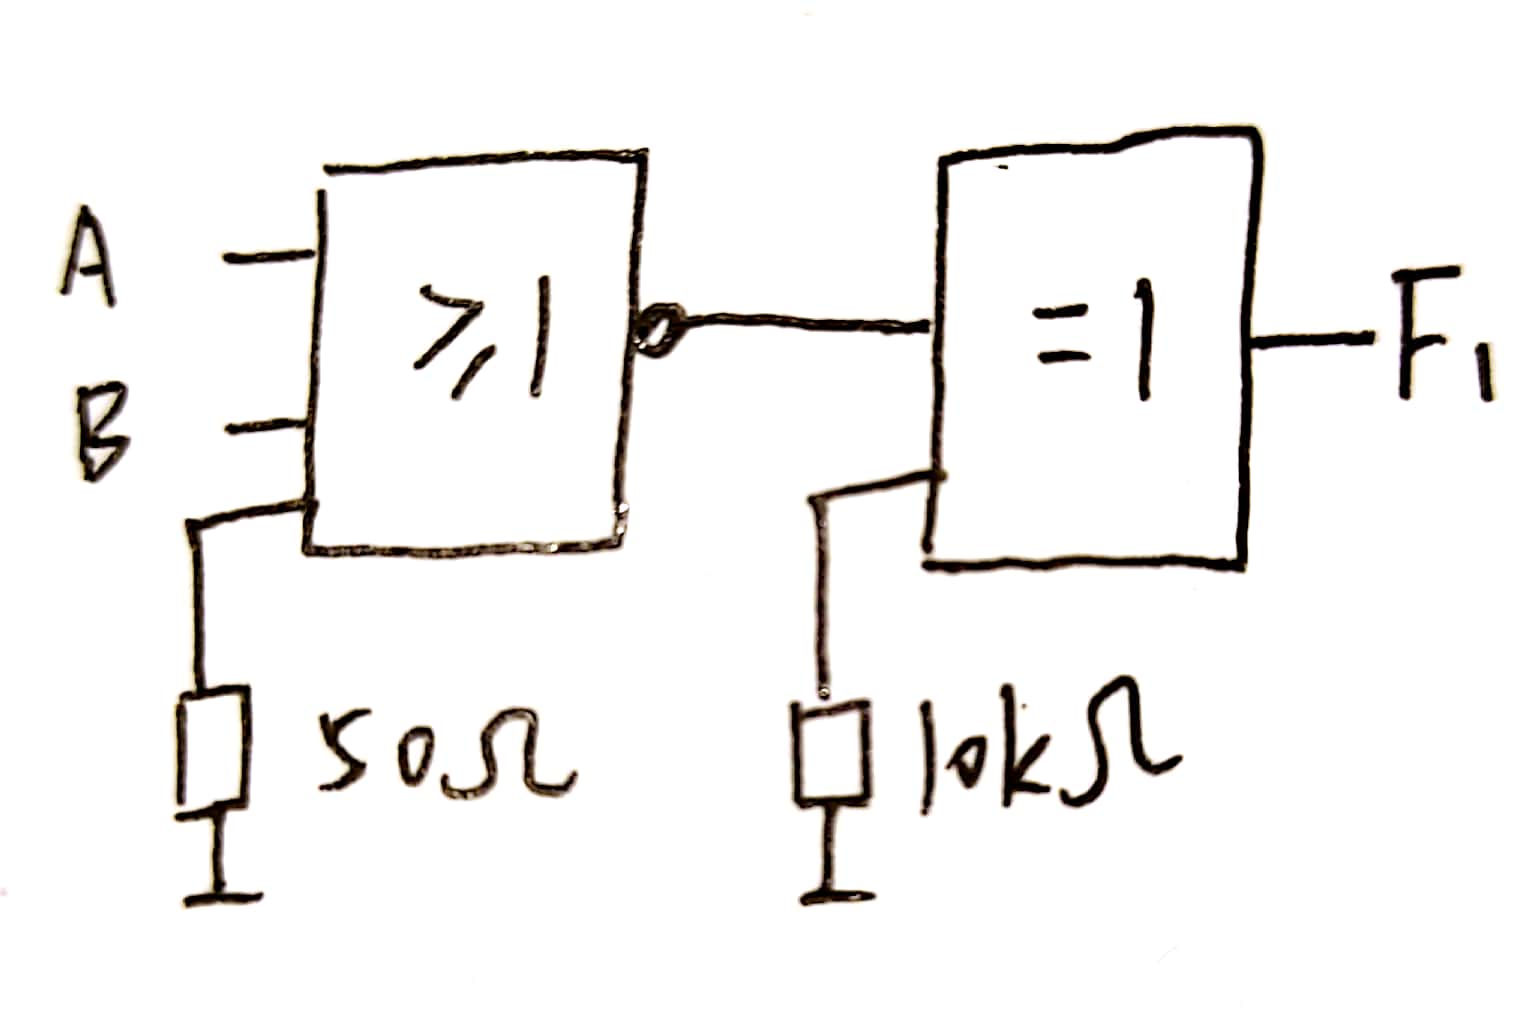
\includegraphics[width=0.3\textwidth]{fig1.jpg}
				\caption{}\label{fig:1}
			}%
			\parbox[t]{0.5\textwidth}{%
				\centering
				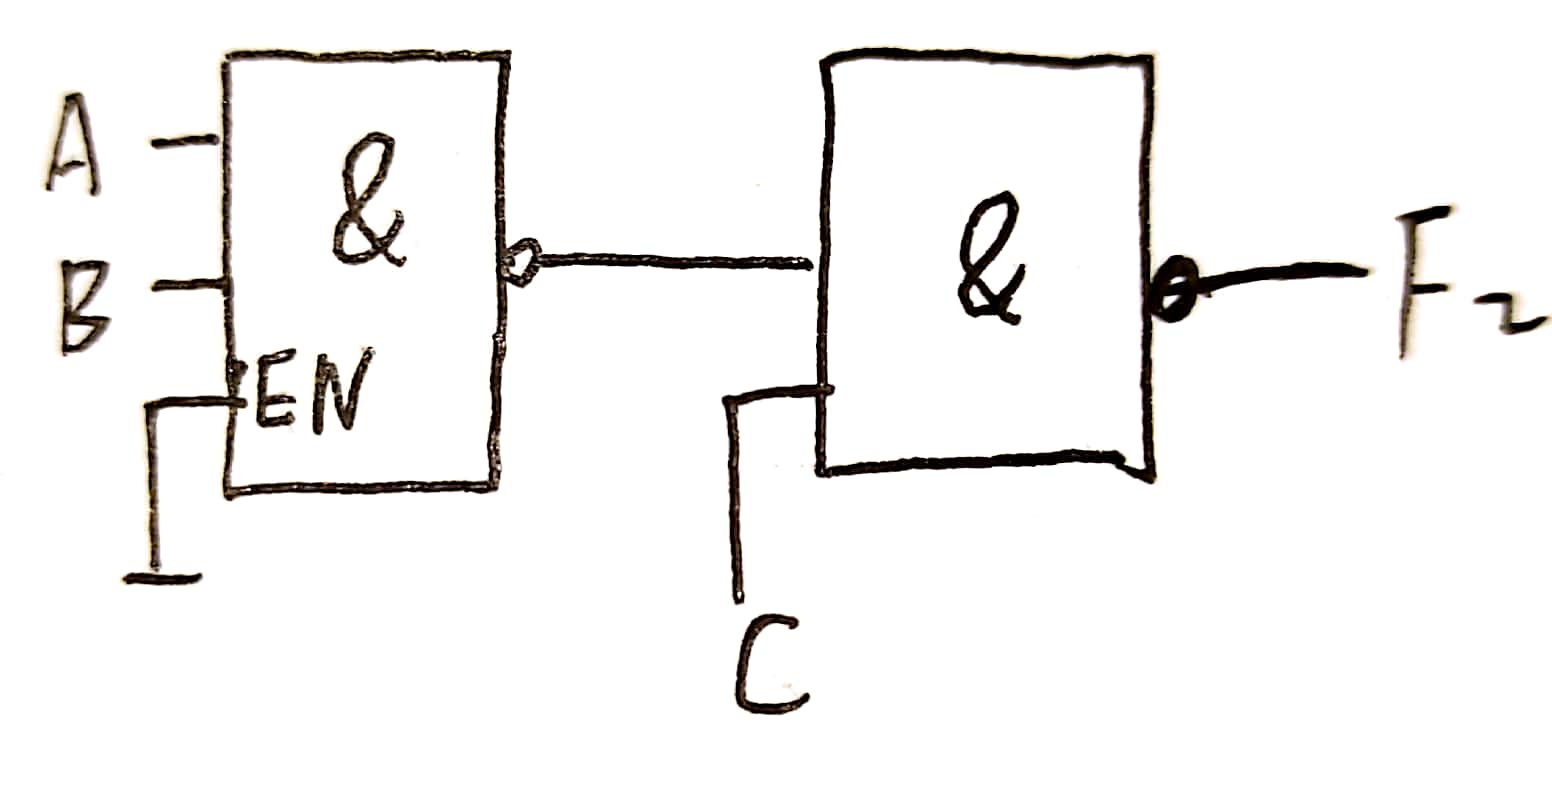
\includegraphics[width=0.3\textwidth]{fig2.jpg}
				\caption{}\label{fig:2}
			}
			\parbox[t]{0.5\textwidth}{%
				\centering
				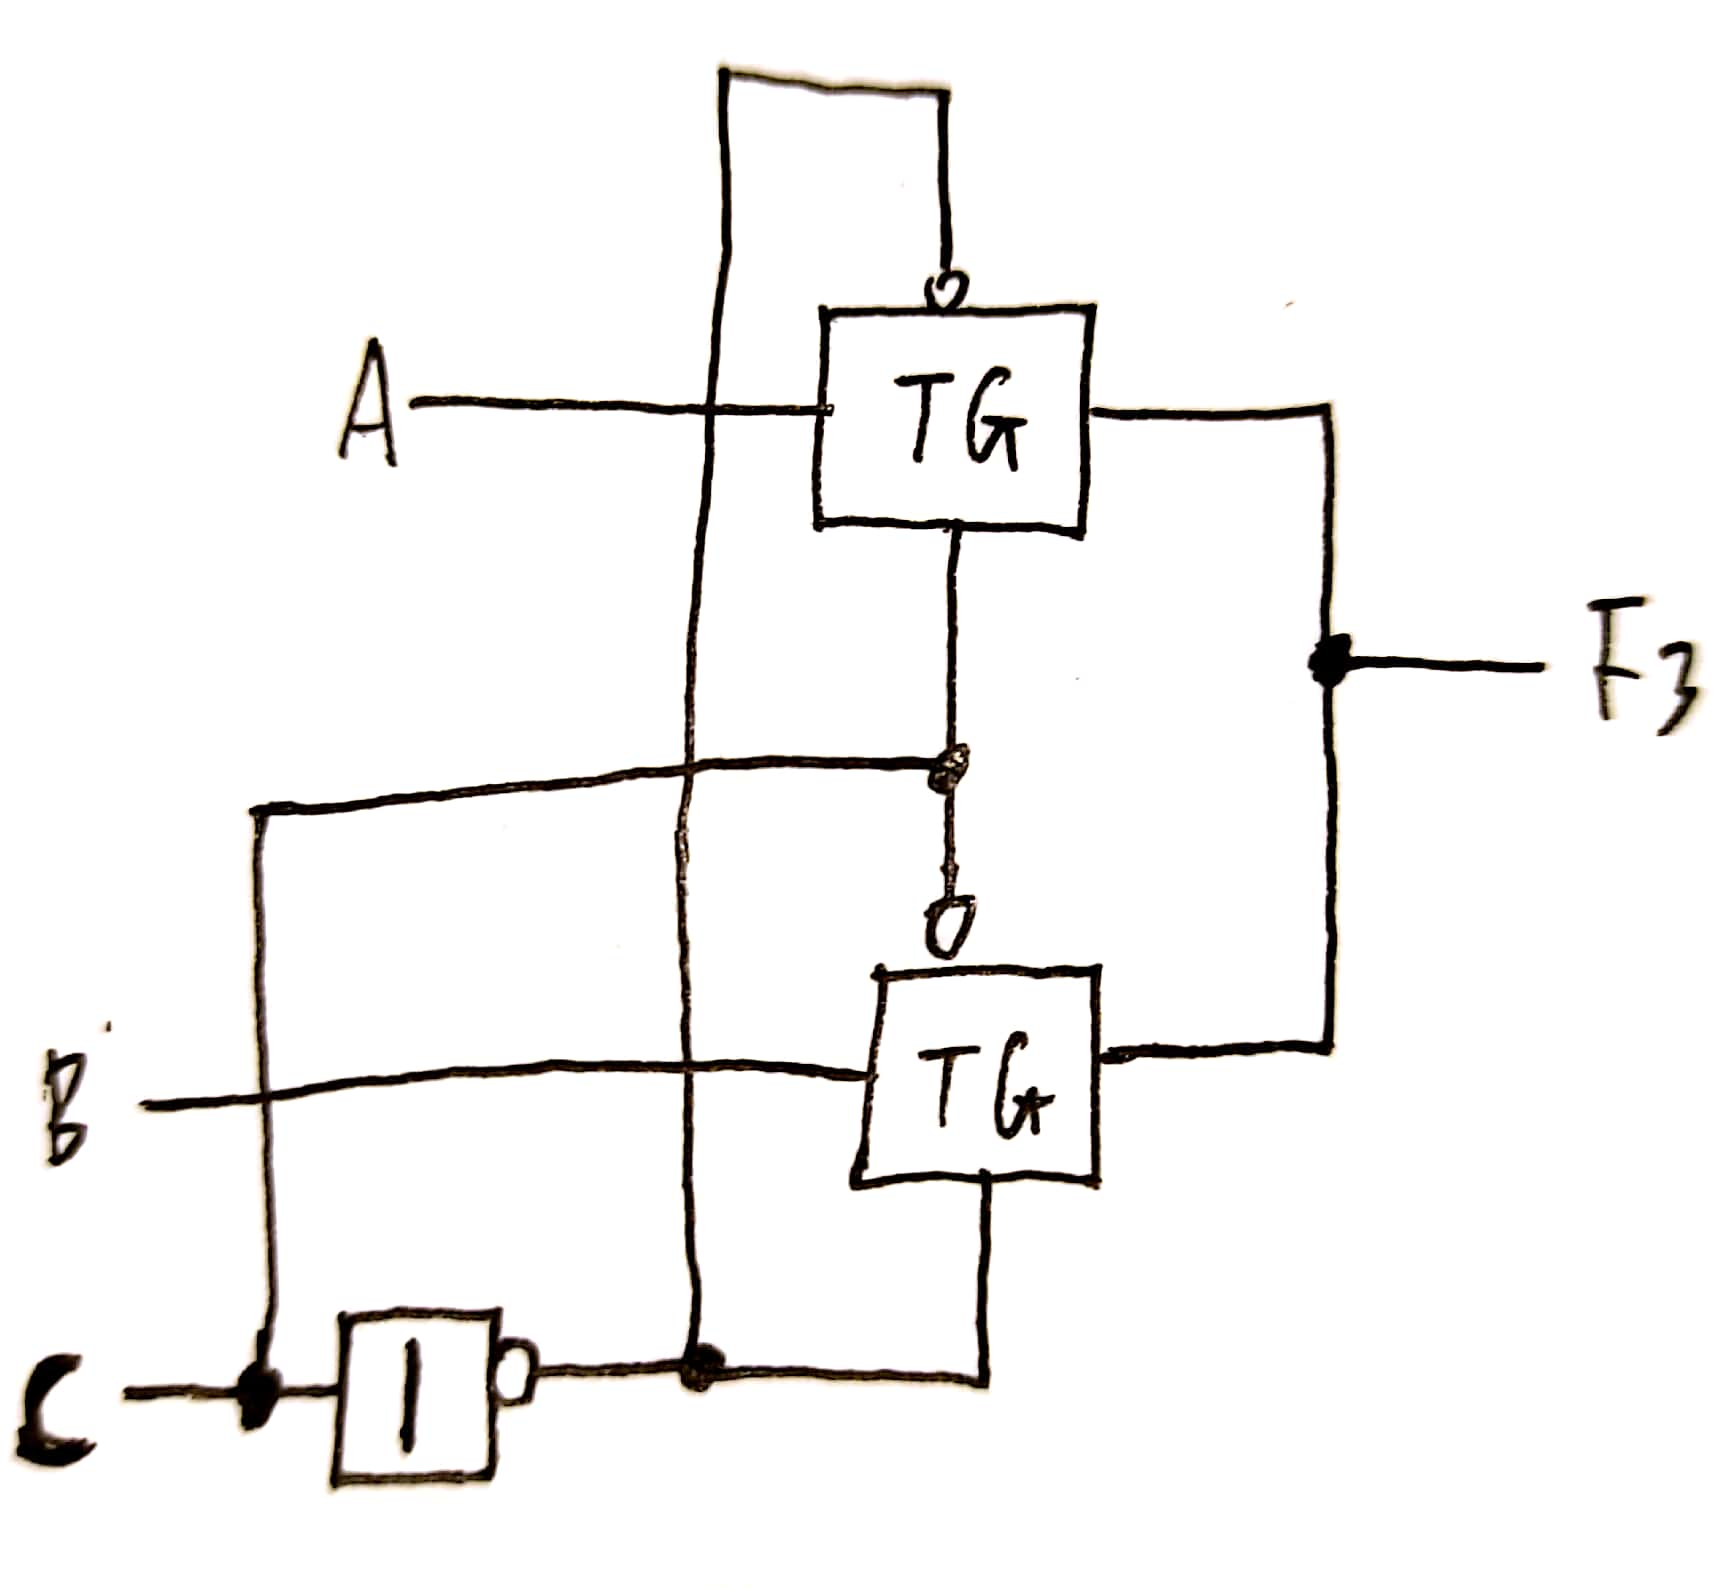
\includegraphics[width=0.3\textwidth]{fig3.jpg}
				\caption{}\label{fig:3}
			}%
		\end{figure}
	\end{ti}

	\begin{ti}[$10$ 分]
		分析逻辑电路
		\begin{inparaenum}
			\item 写输出逻辑表达式
			\item 化最简与或式
			\item 列真值表
			\item 说明逻辑功能
		\end{inparaenum}
		\begin{center}
			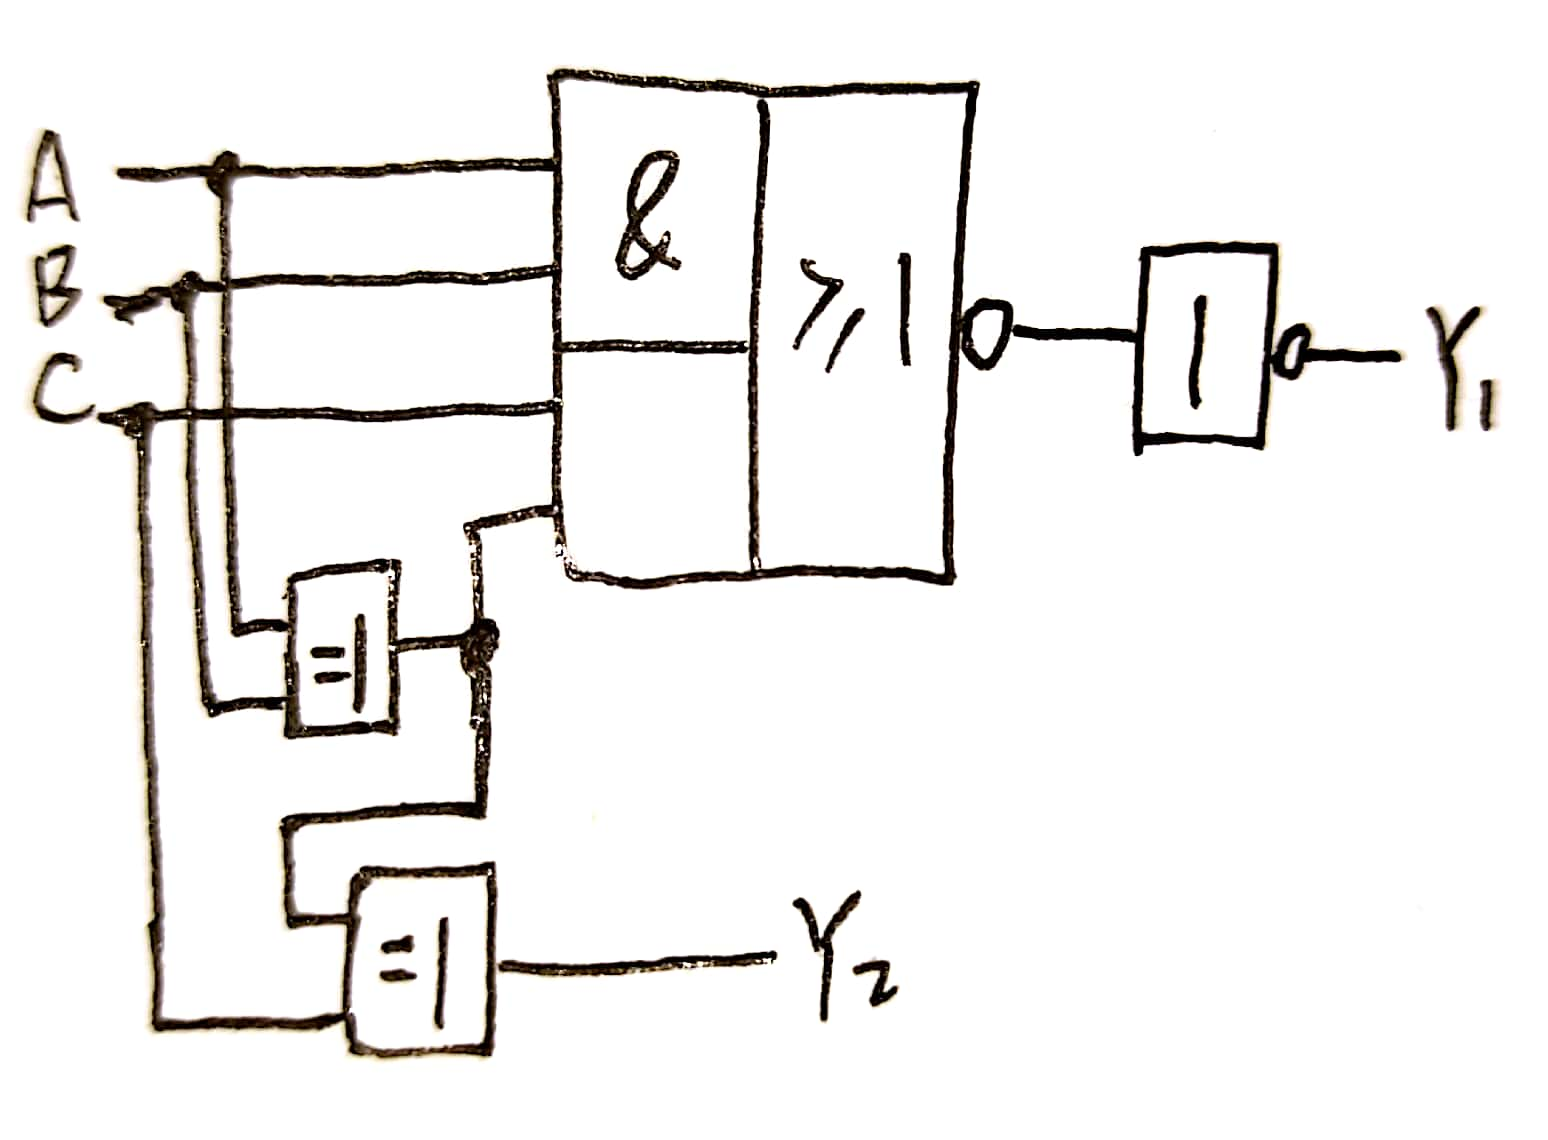
\includegraphics[width=0.3\textwidth]{fig4.jpg}
		\end{center}
	\end{ti}
	
	\begin{ti}[$12$ 分]
		用 8 选 1 数据选择器 74HC151 产生三人表决电路
		\begin{center}
			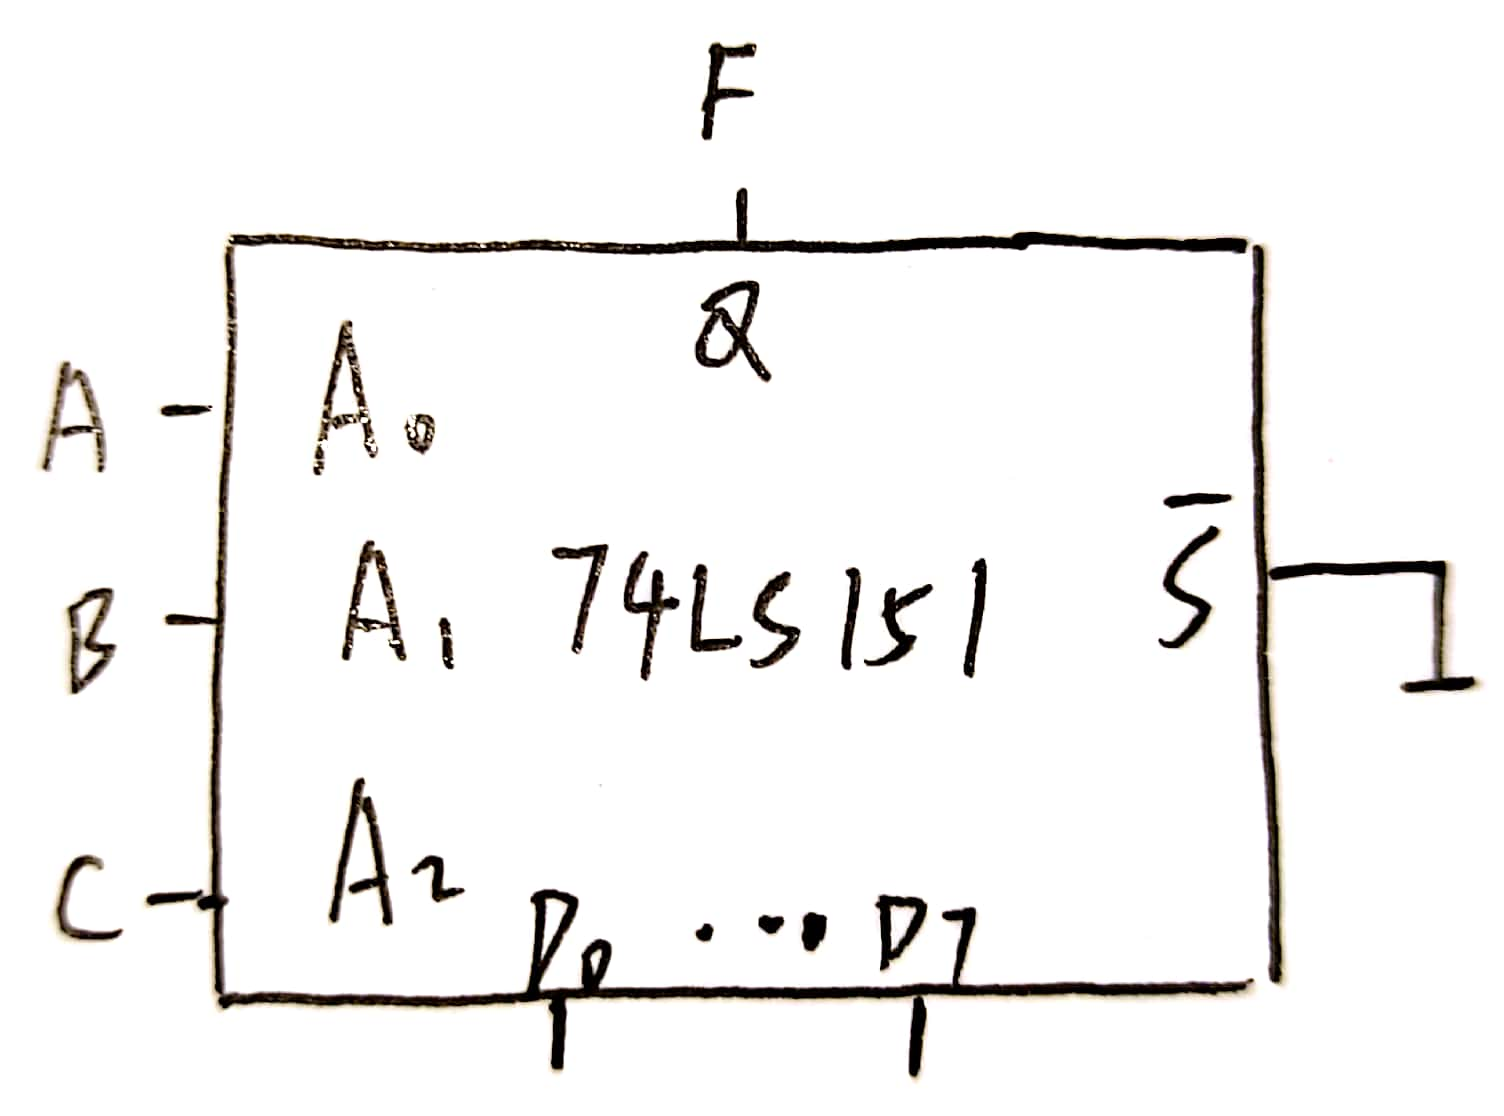
\includegraphics[width=0.4\textwidth]{fig5.jpg}
		\end{center}
	\end{ti}

	\begin{ti}[$12$ 分]
		逻辑电路及 $CP$、$A$ 的电压波形如下图所示,试画出 $Q$ 的波形(初态为“0”)
		\begin{center}
			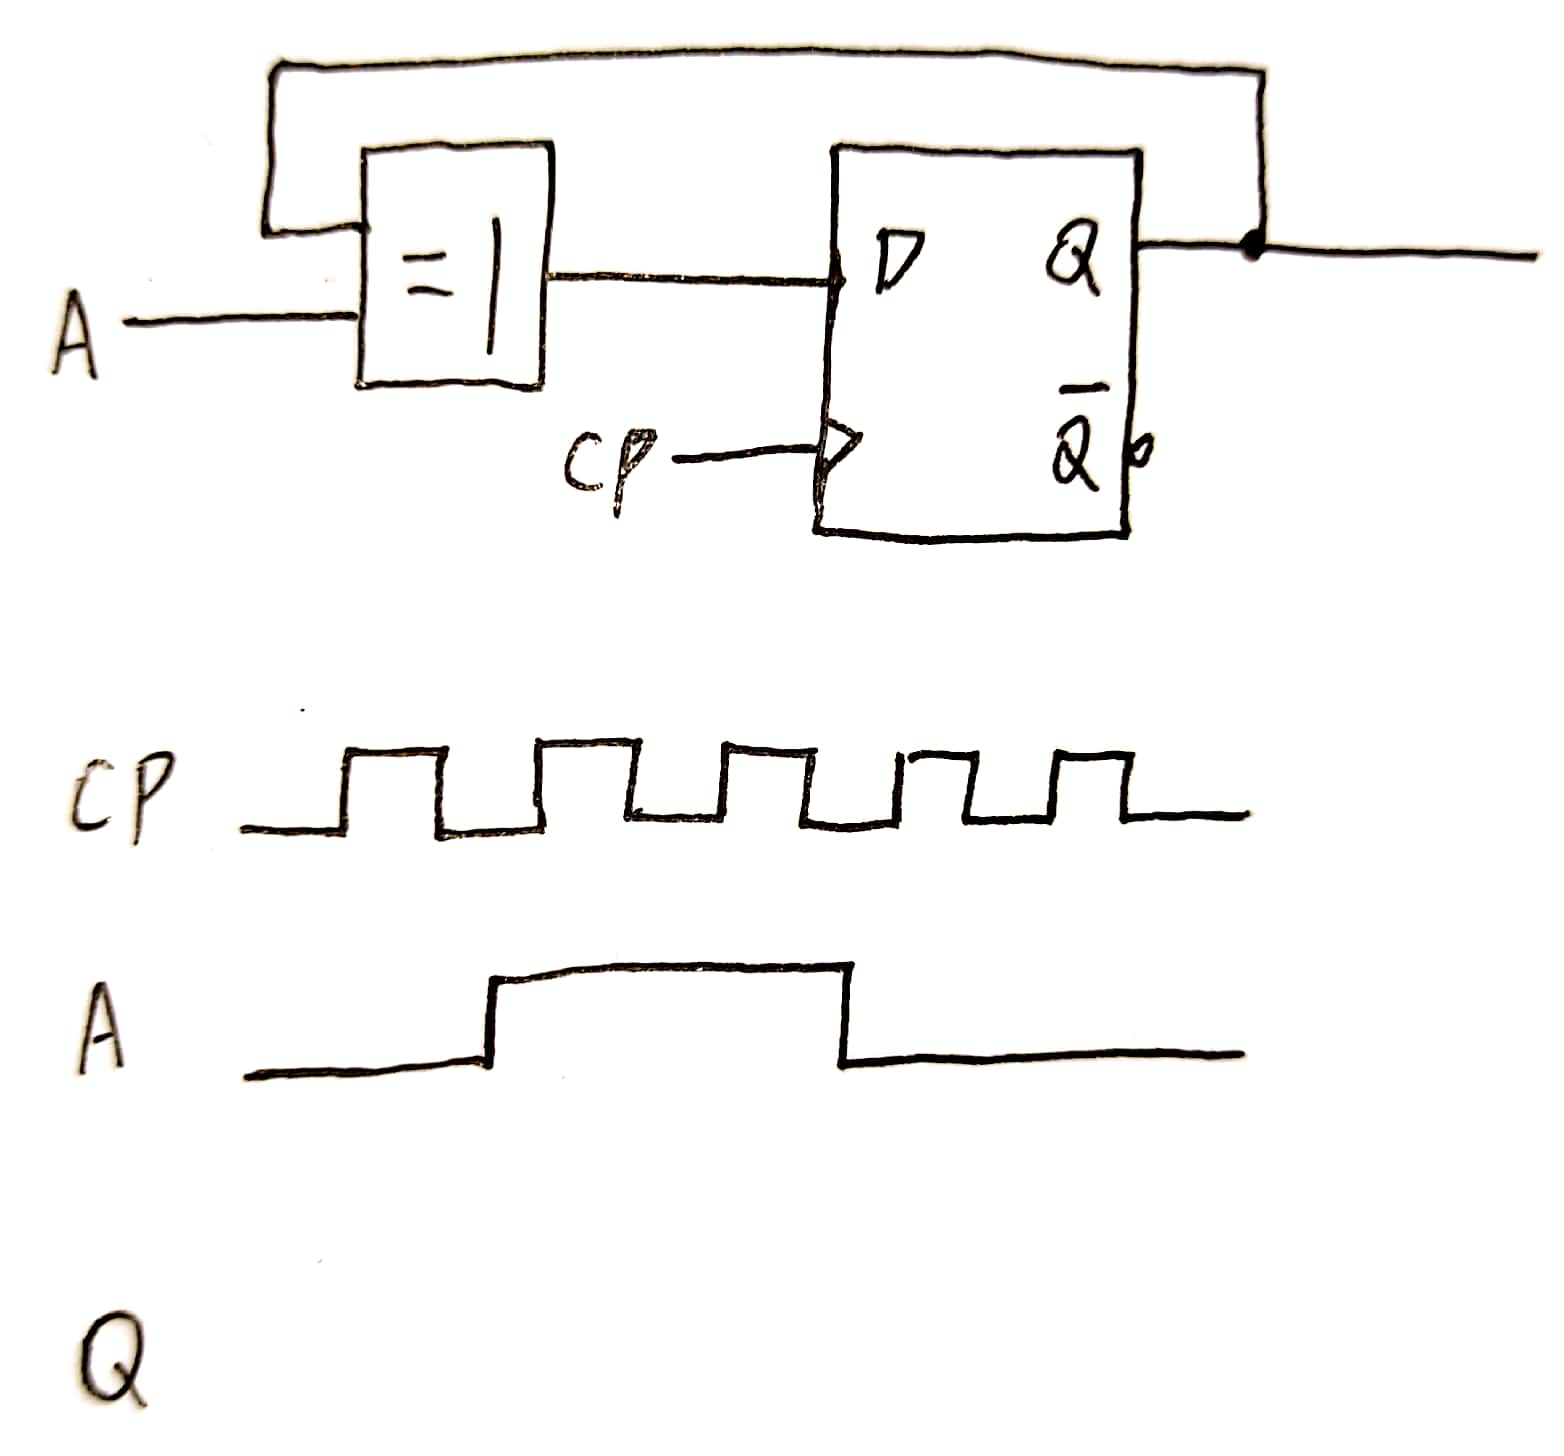
\includegraphics[width=0.4\textwidth]{fig6.jpg}
		\end{center}
	\end{ti}

	\begin{ti}[$12$ 分]
		逻辑电路如下图所示,试求出各个触发器的驱动方程、状态方程及逻辑图的状态表,并说明该电路实现的功能,设初态均为 0
		\begin{center}
			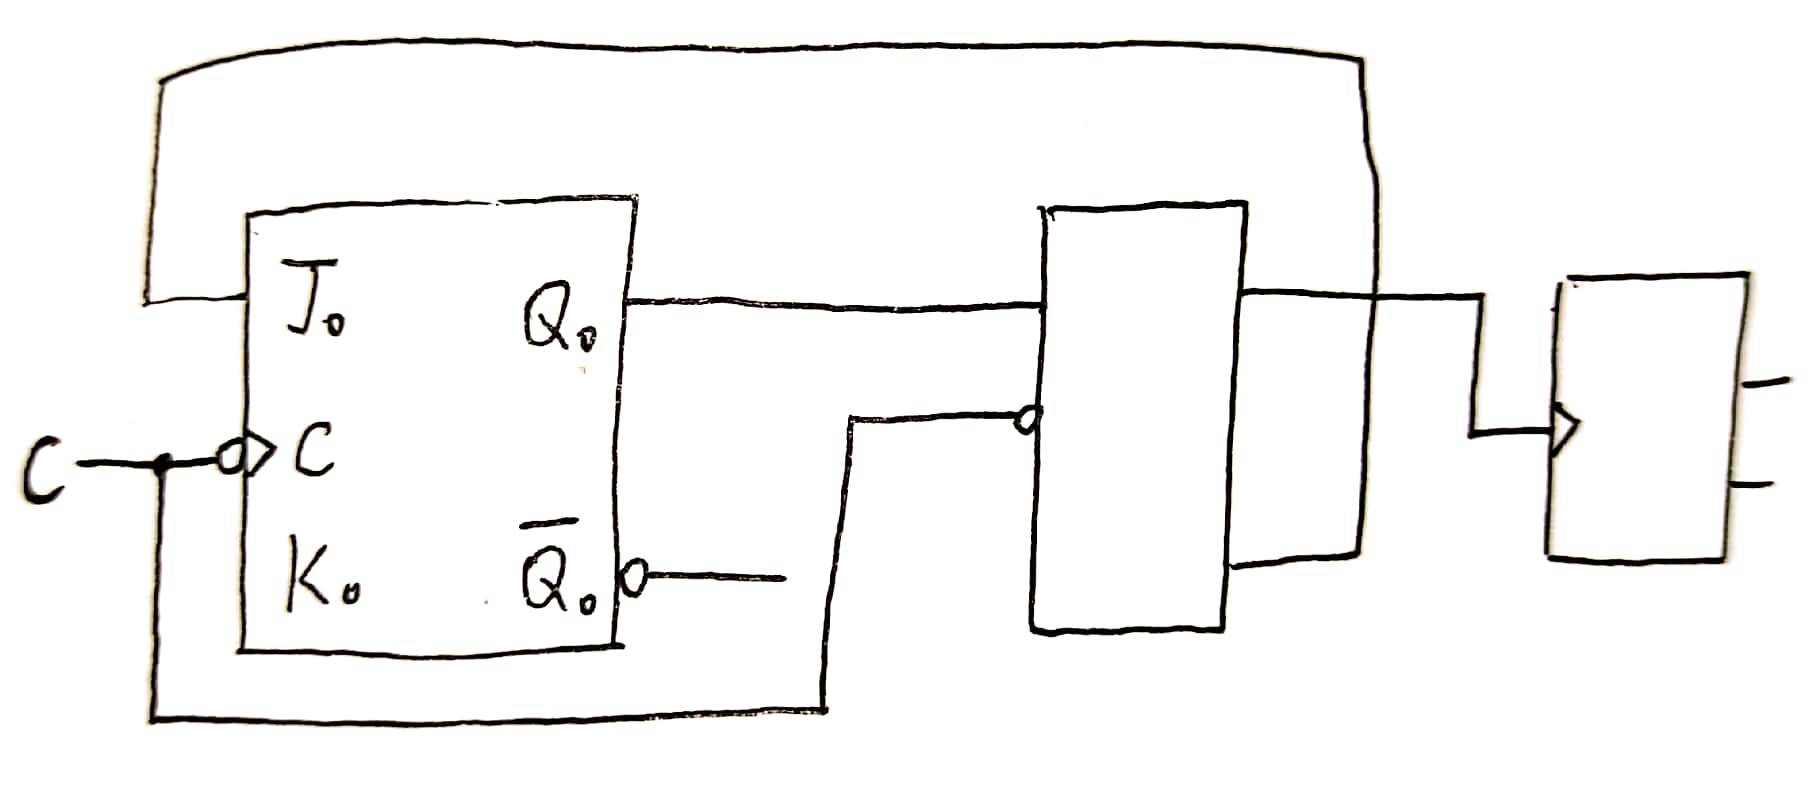
\includegraphics[width=0.6\textwidth]{fig7.jpg}
		\end{center}
	\end{ti}
\end{document}